\clearpage
\subsection{Production}

\subsubsection{scope}
\par{This section provides the detailed use case requirements for the use cases offered by the Production
module.}

\begin{figure}[h]
	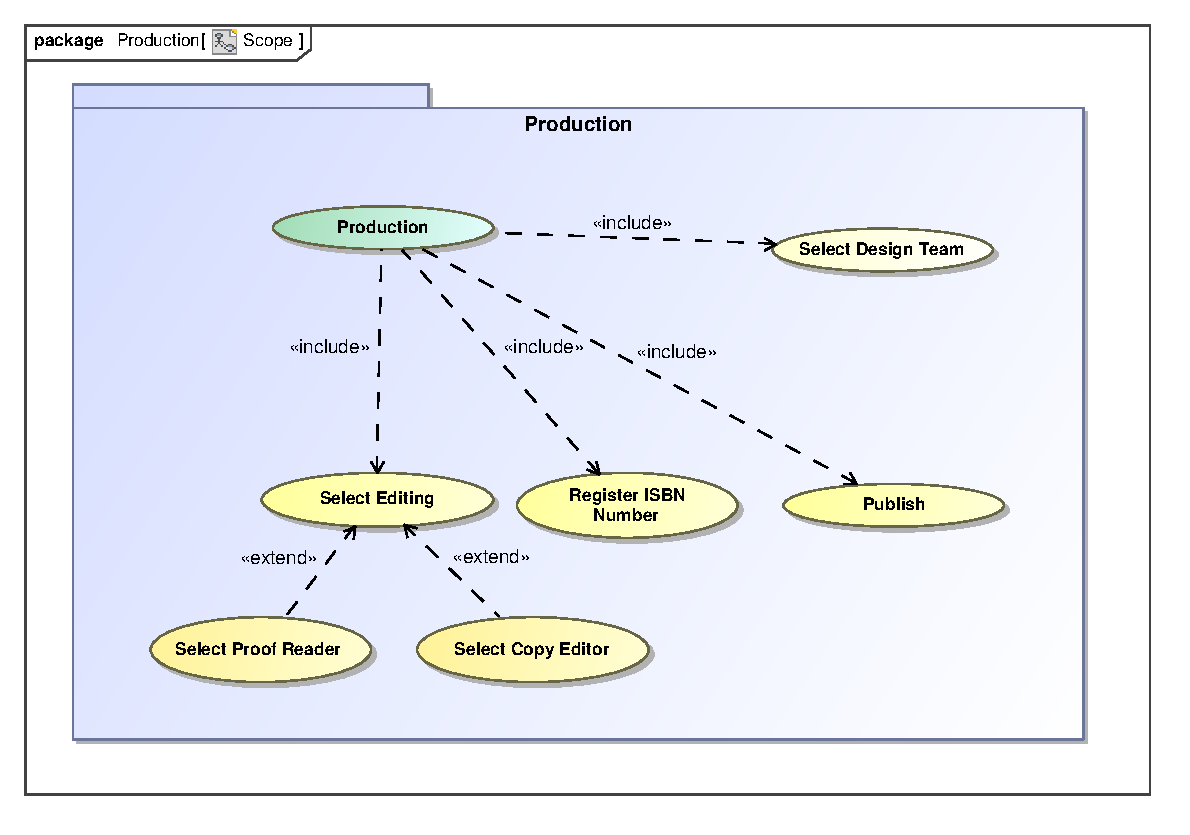
\includegraphics[height=280px, width=500px]{epsImages/Production/Scope.eps}
	\caption{Scope for Production module}
\end{figure}

\newpage
\subsubsection{Use Cases}
\begin{enumerate}
\item \textbf{Register ISBN Number - priority: important}

\par{This use case will allow the user to fill in an application form to register the ISBN number of the manuscript. Most of the inputs on this application form will be auto-completed and an email requesting the ISBN Number will be sent.}

\textbf{Service Contract:} 
Below is a figure of the registerISBNNumber service contract.

\begin{figure}[h]
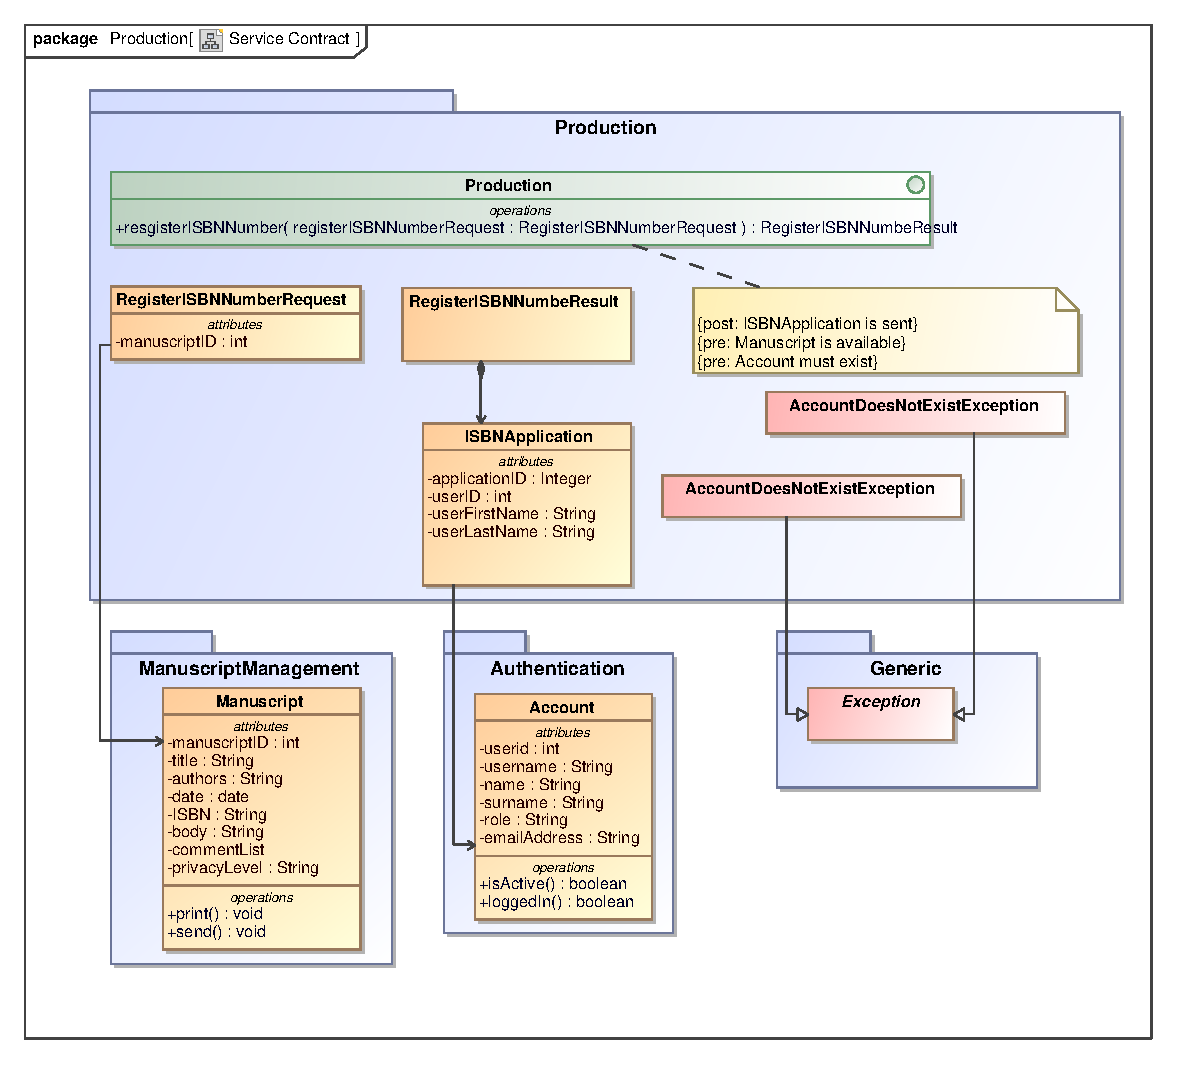
\includegraphics[height=380px, width=500px]{epsImages/Production/RegisterISBNNumber.eps}
\caption{Service contract for registering a manuscript's ISBN number.}
\end{figure}

\newpage
\item \textbf{Select Copy Editor - priority: critical}\\

\par{This use case allows a user to select a copy-editor from the available copy copy-editors registered in the system.}

\clearpage
\textbf{Service Contract:} 
The service contract for selecting a copy editor service is shown in the figure below. The pre-conditions are enforced (raising the appropriate exception should they not be met) and the required copy editor is then notified of the user's request.

\begin{figure}[h]
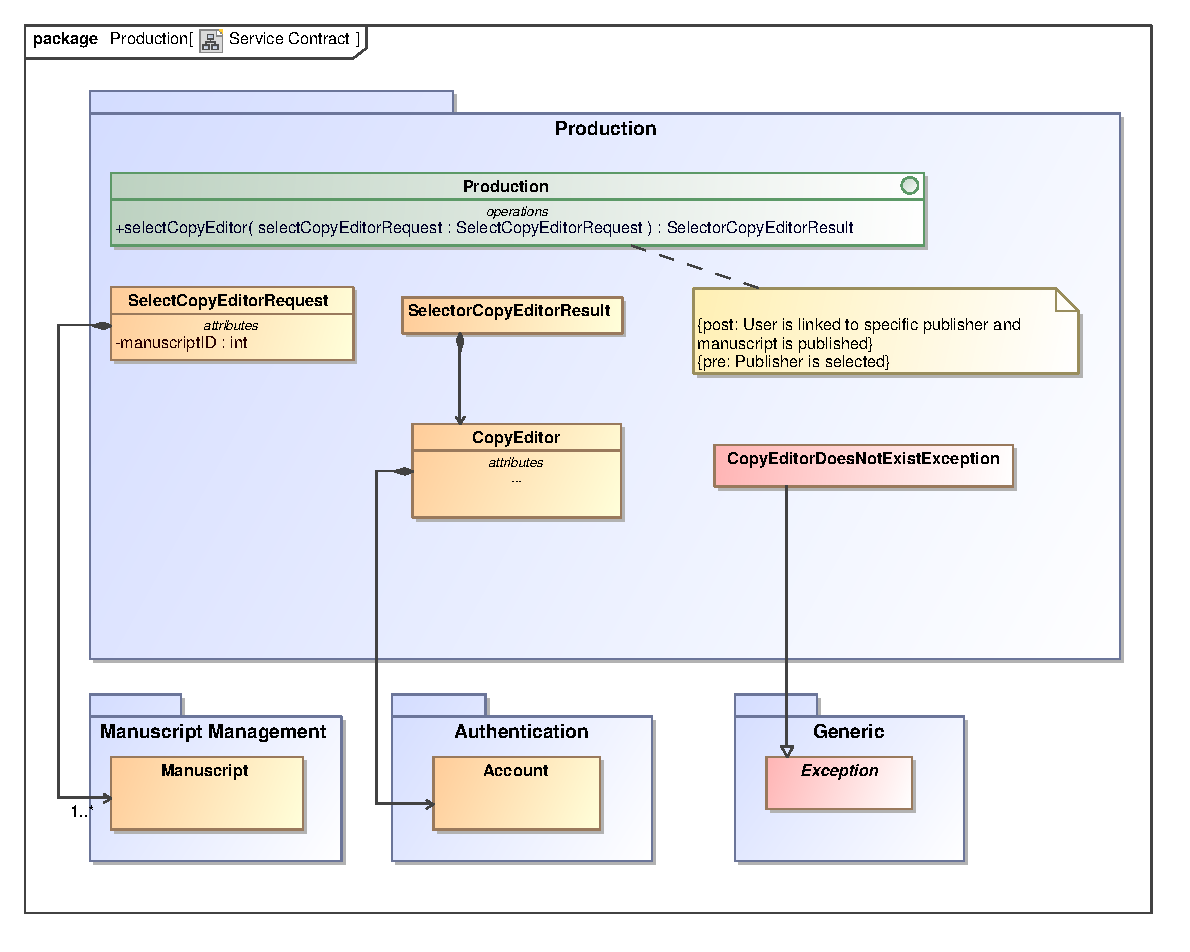
\includegraphics[height=380px, width=500px]{epsImages/Production/SelectCopyEditor.eps}
\caption{Service contract for selecting a copy editor}
\end{figure}

\newpage
\item \textbf{Select Proof Reader – priority: important}\\
\par{This use case allows a user to select a proof reader from the available proof readers registered in the system.}

\textbf{Service Contract:} 
The service contract for selecting a proof reader service is shown in the figure below. The pre-conditions are enforced (raising the appropriate exception should they not be met) and the required proof reader is then notified of the user's request.

\begin{figure}[h]
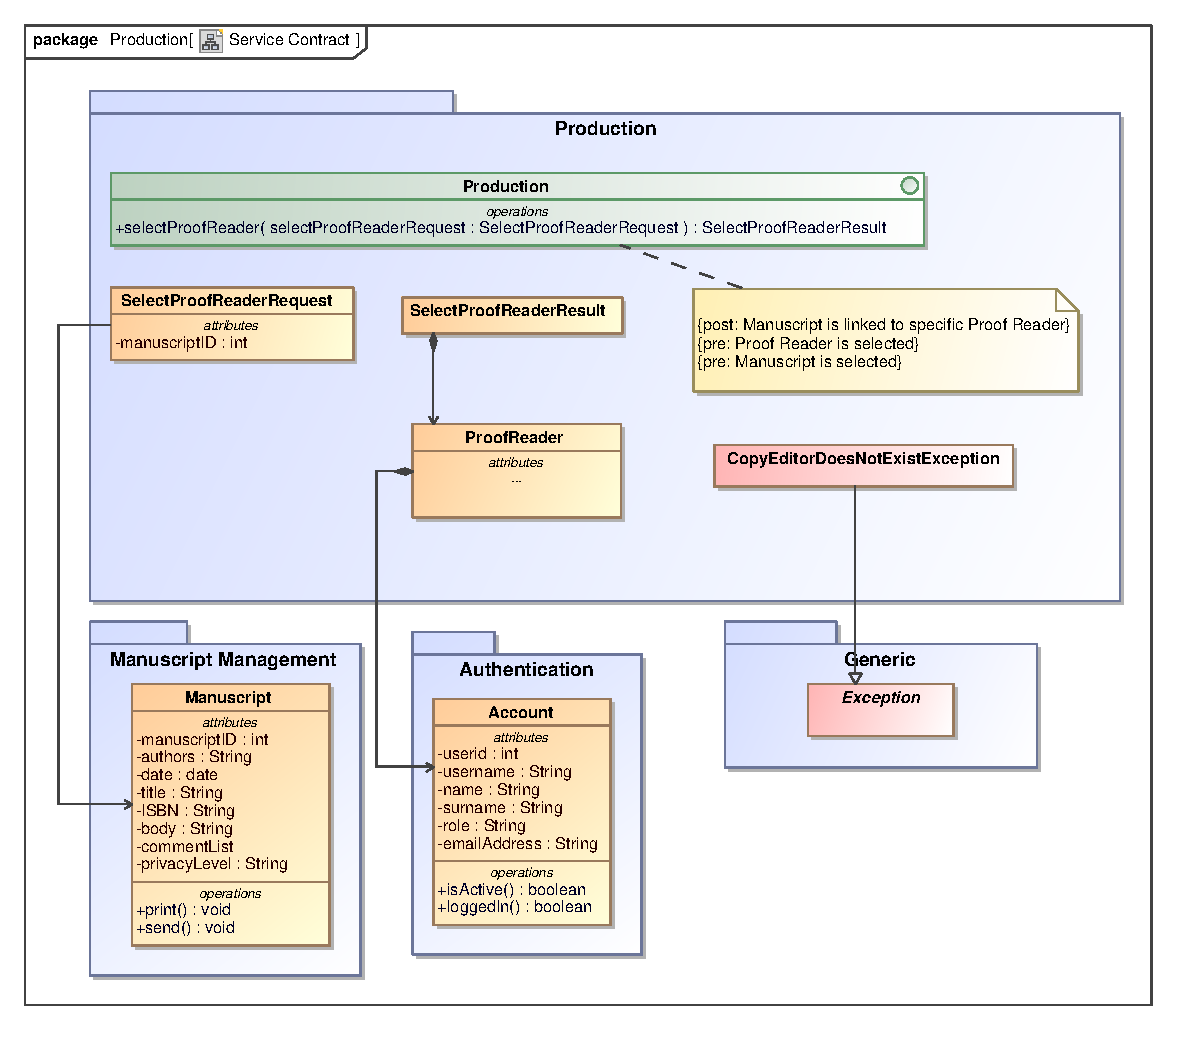
\includegraphics[height=380px, width=500px]{epsImages/Production/SelectProofReader.eps}
\caption{Service contract for selecting a proof reader}
\end{figure}

\newpage
\item \textbf{Select Design Team – priority: important}\\
\par{This use case allows a user to select, from the registered designers, a design team that will be resposible for the book cover and styling.}

\textbf{Service Contract:} 
The service contract for the selectDesignTeam service is shown in figure below. The pre-conditions are enforced (raising the appropriate exception should they not be met) and the required design team is notified.

\begin{figure}[h]
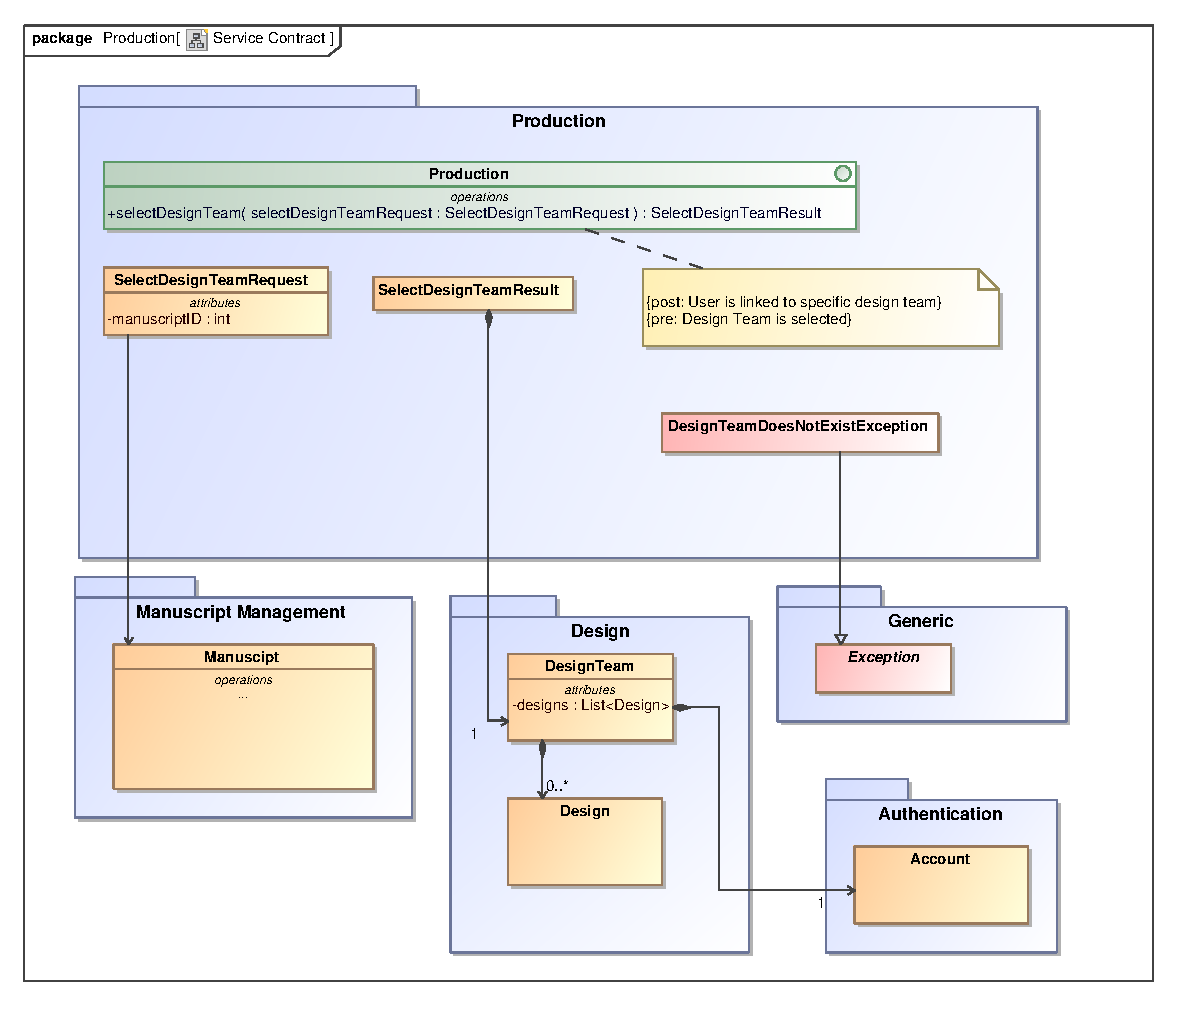
\includegraphics[height=380px, width=500px]{epsImages/Production/SelectDesignTeam.eps}
\caption{Service contract for selecting a design team}
\end{figure}


\newpage
\item \textbf{Publish - priority: critical}
\par{This use case allows an agent or an editorial to select a publisher and request that the final manuscript be published.}

\textbf{Service Contract:} 
The service contract for publish is shown in the diagram below. The pre-conditions are enforced (raising the appropriate exception should they not be met) and a preferred publisher is notified of the publishing request.

\begin{figure}[h]
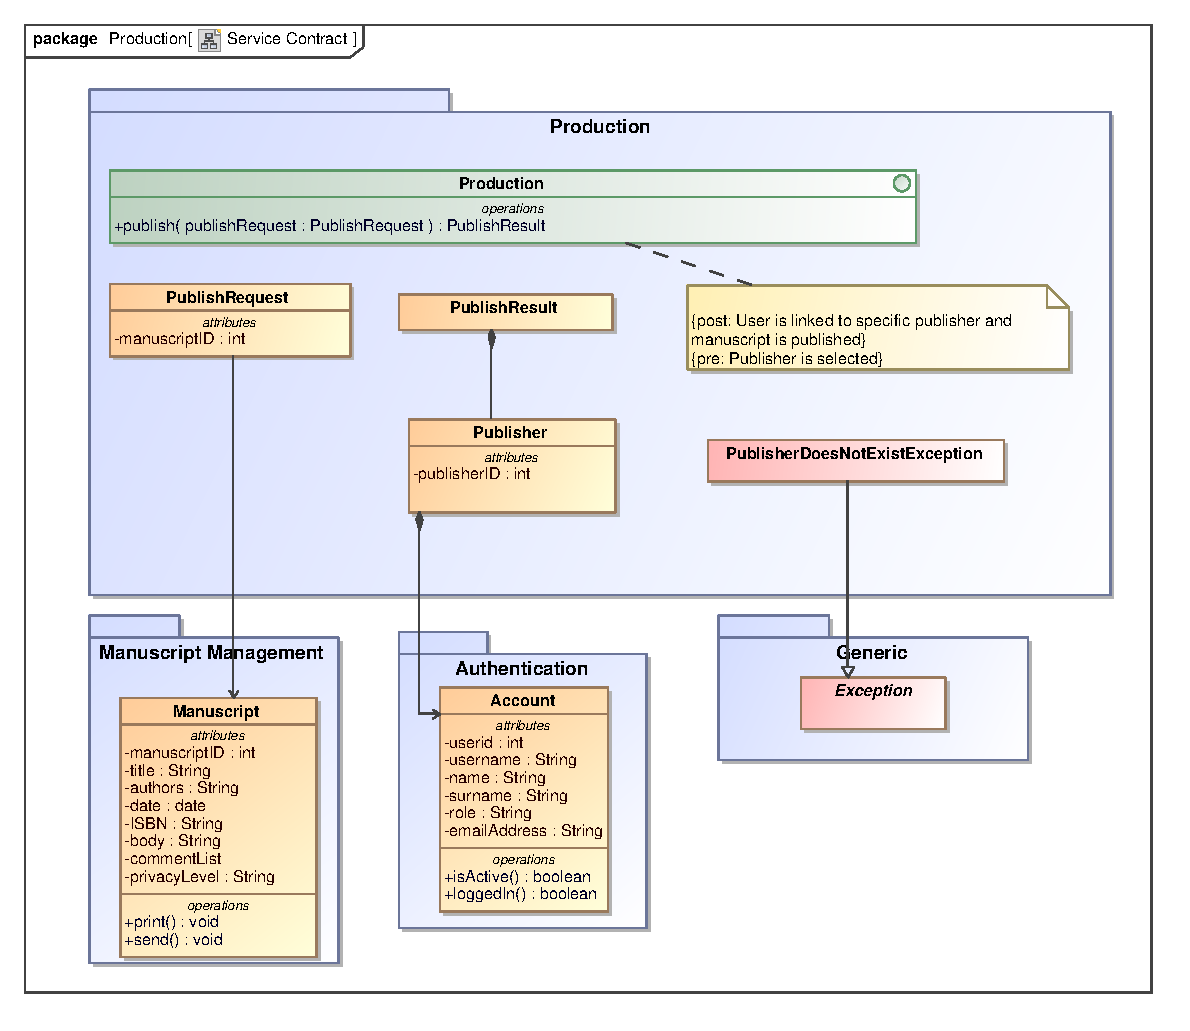
\includegraphics[height=380px, width=500px]{epsImages/Production/Publish.eps}
\caption{Service contract for evaluating a publish}
\end{figure}

 \newpage
\textbf{Domain Model:} Below is a figure for the domain model of manuscript management. 

\begin{figure}[h]
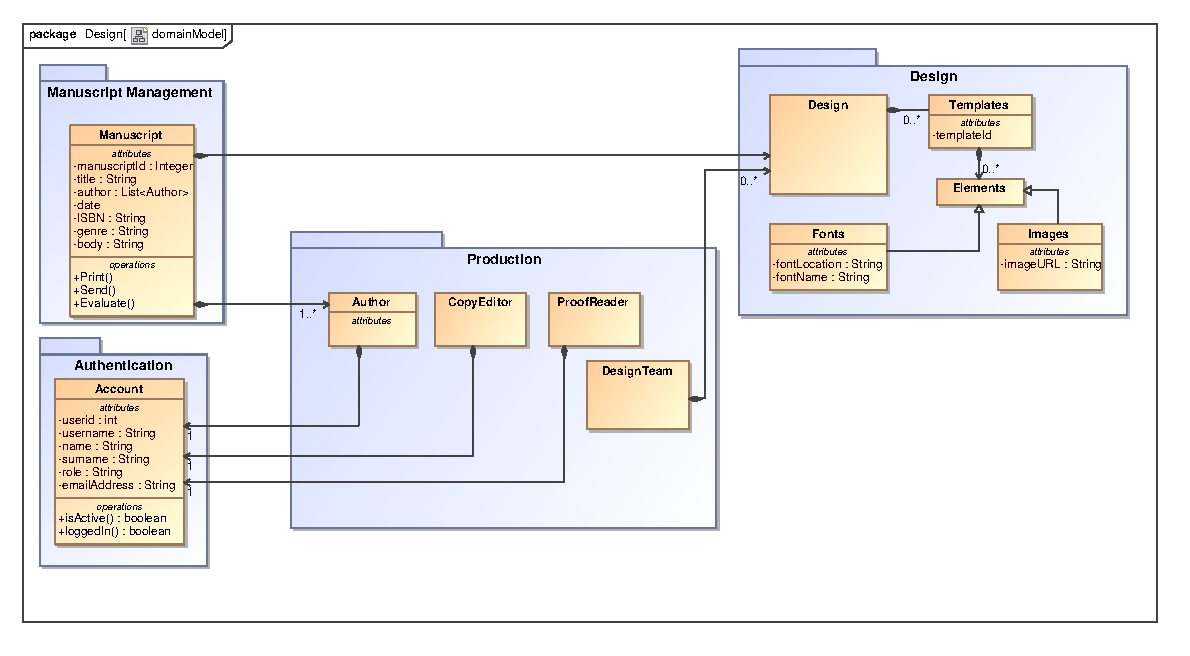
\includegraphics[height=380px, width=500px]{epsImages/DomainModels/ProductionDomainModel.eps}
\caption{Domain model for managing a manuscript}
\end{figure}


\end{enumerate}
